% ------------------------------------------------------------
\section{Case study: the tent (piecewise-linear) profile}
\label{sec:tent}
% ------------------------------------------------------------

\subsection{The profile and its algebraic properties}

We now specialise to the tent profile~\eqref{eq:tent},
\[
D(x)\;=\;D_0 \;+\; D_1\!\left(1-\frac{|x|}{\pi}\right).
\]
On the half-interval $[0,\pi]$, $D(x)=\alpha-\beta x$ with
$\alpha\equiv D_0+D_1=D(0)$ and $\beta\equiv D_1/\pi$; equivalently,
$D(\pi)=D_0$.  For $D_1>0$ the diffusivity peaks at the trap; for $D_1<0$ it
has a dip at the trap.  We restrict to $|D_1|<D_0$ to keep $D(x)>0$ everywhere.
The profile and a few representative choices of $D_1$ are displayed in
Figure~\ref{fig:tent-profile}.

\begin{figure}[!ht]
\centering
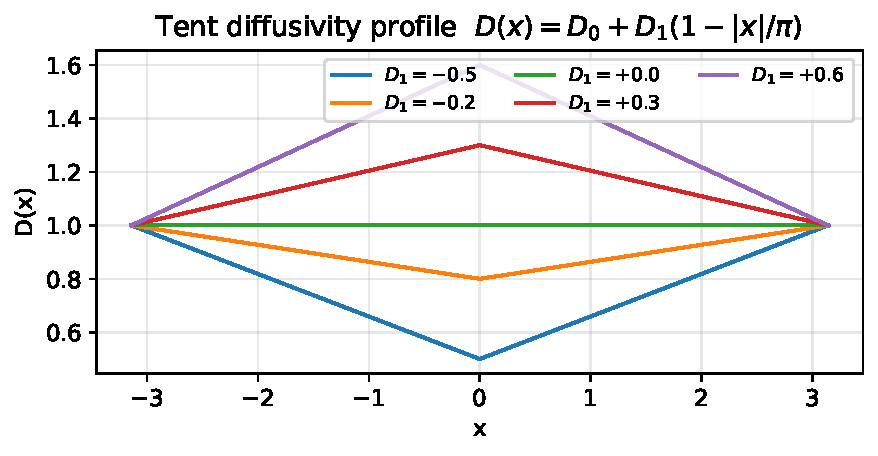
\includegraphics[width=0.66\linewidth]{files/fig_tent_profile.pdf}
\caption{Tent diffusivity profile $D(x)=D_0+D_1(1-|x|/\pi)$ for several values
of $D_1$ ($D_0=1$).  Positive $D_1$ produces a peak at the trap $x=0$; negative
$D_1$ produces a dip.  The profile is continuous but not differentiable at
$x=0$.}
\label{fig:tent-profile}
\end{figure}

\subsection{Explicit evaluation of \texorpdfstring{$T(x)$}{T(x)}}

Substitute $D(y)=\alpha-\beta y$ into \eqref{eq:T-final} and compute the
integral explicitly.  Let $u=\alpha-\beta y$, so $y=(\alpha-u)/\beta$ and
$dy=-du/\beta$; further, $\pi-y=\pi-(\alpha-u)/\beta=(\pi\beta-\alpha+u)/\beta$.
Note that $\pi\beta=D_1$, so $\pi\beta-\alpha=D_1-(D_0+D_1)=-D_0$.  Therefore
\[
\int_0^x\!\frac{\pi-y}{\alpha-\beta y}\,dy
=\int_{\alpha}^{D(x)}\!\frac{(u-D_0)/\beta}{u}\,\frac{-du}{\beta}
=-\frac{1}{\beta^2}\!\int_{\alpha}^{D(x)}\!\left(1-\frac{D_0}{u}\right)du,
\]
where we have used $(u-D_0)/u=1-D_0/u$.  The inner integral is elementary:
\[
\int_{\alpha}^{D(x)}\!\left(1-\frac{D_0}{u}\right)du
=\bigl[u-D_0\ln u\bigr]_{\alpha}^{D(x)}
=\bigl(D(x)-\alpha\bigr) - D_0\ln\!\frac{D(x)}{\alpha}.
\]
Combining with the prefactor $-1/\beta^2=-\pi^2/D_1^2$,
\begin{equation}
\int_0^x\!\frac{\pi-y}{D(y)}\,dy
\;=\;\frac{\pi^2}{D_1^2}\left[\,D(0)-D(x) \;+\; D_0\ln\!\frac{D(x)}{D(0)}\,\right],
\qquad x\in[0,\pi].
\label{eq:tent-T-integral}
\end{equation}
The full MFPT is therefore
\begin{equation}
\boxed{\;
T(x)\;=\;\frac{2\pi}{\kappa}\;+\;\frac{\pi^2}{D_1^2}\!\left[\,D_0\ln\!\frac{D(x)}{D(0)}\;+\;D(0)-D(x)\,\right],
\qquad x\in[-\pi,\pi].
\;}\label{eq:T-tent}
\end{equation}

Several sanity checks:
\begin{enumerate}[label=(\roman*)]
\item At $x=0$, $D(x)=D(0)$, the bracket vanishes, and $T(0)=2\pi/\kappa$.
\item At $x=\pm\pi$, $D(x)=D_0$ and
\[
T(\pm\pi)\;=\;\frac{2\pi}{\kappa}\;+\;\frac{\pi^2}{D_1^2}\!\left[\,D_1 - D_0\ln\!\frac{D_0+D_1}{D_0}\,\right],
\]
which is positive for all $|D_1|<D_0$ (Taylor-expanding the log near $D_1=0$
gives a leading $D_1^2/(2D_0)$).
\item As $D_1\to 0$, using $\ln(1+z)=z-z^2/2+z^3/3-\cdots$,
\[
D_0\ln\frac{D_0+D_1}{D_0}=D_0\!\left(\frac{D_1}{D_0}-\frac{D_1^2}{2D_0^2}+\cdots\right)
=D_1-\frac{D_1^2}{2D_0}+\cdots,
\]
so the bracket at $x=\pi$ becomes $D_1^2/(2D_0)+O(D_1^3)$ and
$T(\pi)\to 2\pi/\kappa+\pi^2/(2D_0)$.  This agrees with the homogeneous answer
$T(\pi)=2\pi/\kappa+[\pi\cdot\pi-\pi^2/2]/D_0=2\pi/\kappa+\pi^2/(2D_0)$
obtained by substituting $D(y)\equiv D_0$ into \eqref{eq:T-final}. \checkmark
\end{enumerate}

\subsection{Spatial average \texorpdfstring{$\langle T\rangle$}{<T>}}

By~\eqref{eq:T-avg-general} the travel contribution is
\[
\Delta\!\langle T\rangle_{\rm trav}
=\frac{1}{\pi}\int_0^\pi\!\frac{(\pi-y)^2}{D(y)}\,dy.
\]
Substituting $u=\pi-y$ (so $y=\pi-u$, $D(y)=D_0+D_1 u/\pi$, $dy=-du$, limits
flip),
\[
\int_0^\pi\!\frac{(\pi-y)^2}{D(y)}\,dy
=\int_0^\pi\!\frac{u^2}{D_0+D_1 u/\pi}\,du.
\]
Next let $v=D_0+D_1 u/\pi$, so $u=\pi(v-D_0)/D_1$, $du=(\pi/D_1)\,dv$, and the
limits become $v\in[D_0,D_0+D_1]$:
\[
\int_0^\pi\!\frac{u^2}{v}\,du
=\frac{\pi^3}{D_1^3}\!\int_{D_0}^{D_0+D_1}\!\frac{(v-D_0)^2}{v}\,dv
=\frac{\pi^3}{D_1^3}\!\int_{D_0}^{D_0+D_1}\!\left(v - 2D_0 + \frac{D_0^2}{v}\right)dv.
\]
The remaining integral is elementary:
\begin{align*}
\int_{D_0}^{D_0+D_1}\!\left(v-2D_0+\frac{D_0^2}{v}\right)dv
&= \left[\frac{v^2}{2}-2D_0 v+D_0^2\ln v\right]_{D_0}^{D_0+D_1}\\
&=\frac{(D_0+D_1)^2-D_0^2}{2} - 2D_0 D_1 + D_0^2\ln\!\frac{D_0+D_1}{D_0}\\
&=D_0 D_1+\frac{D_1^2}{2} - 2D_0 D_1 + D_0^2\ln\!\frac{D_0+D_1}{D_0}\\
&=\frac{D_1^2}{2}-D_0 D_1+D_0^2\ln\!\frac{D_0+D_1}{D_0}.
\end{align*}
Dividing by $\pi$ to convert to the average,
\begin{equation}
\boxed{\;
\langle T\rangle\;=\;\frac{2\pi}{\kappa}
\;+\;\frac{\pi^2}{D_1^3}\!\left[\frac{D_1^2}{2}-D_0 D_1+D_0^2\ln\!\frac{D_0+D_1}{D_0}\right].
\;}\label{eq:T-avg-tent}
\end{equation}

\paragraph{Homogeneous limit $D_1\to 0$.}
Using $\ln(1+z)=z-z^2/2+z^3/3-z^4/4+O(z^5)$ with $z=D_1/D_0$,
\[
D_0^2\ln\!\frac{D_0+D_1}{D_0}=D_0 D_1-\frac{D_1^2}{2}+\frac{D_1^3}{3D_0}-\frac{D_1^4}{4D_0^2}+O(D_1^5),
\]
so
\[
\frac{D_1^2}{2}-D_0 D_1+D_0^2\ln\!\frac{D_0+D_1}{D_0}
=\frac{D_1^3}{3D_0}-\frac{D_1^4}{4D_0^2}+O(D_1^5).
\]
Dividing by $D_1^3$ gives $1/(3D_0)-D_1/(4D_0^2)+O(D_1^2)$, so
$\langle T\rangle\to 2\pi/\kappa+\pi^2/(3D_0)$, which is the homogeneous
baseline (constant $D=D_0$). \checkmark

\paragraph{Monotonicity in $D_1$.}
Differentiating \eqref{eq:T-avg-tent} term-by-term,
\[
\frac{\partial\langle T\rangle}{\partial D_1}
=-\frac{1}{\pi}\!\int_0^\pi\!\frac{(\pi-y)^2}{D(y)^2}\cdot\frac{\partial D}{\partial D_1}\,dy
=-\frac{1}{\pi}\!\int_0^\pi\!\frac{(\pi-y)^2\,(1-y/\pi)}{D(y)^2}\,dy<0
\]
because the integrand is strictly positive on $(0,\pi)$.  So with $\kappa$
constant, $\langle T\rangle$ is strictly decreasing in $D_1$: the MFPT is
minimised by making $D(0)$ as large as possible (equivalently: concentrating
the mobility at the trap).  This is easy to understand: the travel integrand
$(\pi-y)^2/D(y)$ is heavily weighted near $y=0$, and the tent profile with
$D_1>0$ raises $D$ precisely where the integrand is largest.
